\documentclass[12pt,letterpaper]{article}

% --- Paquetes de Idioma y Formato ---
\usepackage[spanish,es-tabla]{babel} % Idioma español y "Tabla" en vez de "Cuadro"
% Se amplia 'top' a 4cm y 'headheight' a 75pt para darle espacio suficiente al logo de 3.5cm de ancho
\usepackage[top=4cm, bottom=2.5cm, left=2.5cm, right=2.5cm, headheight=75pt, headsep=0.8cm]{geometry}

% --- Encabezados y Pies de Página ---
\usepackage{fancyhdr}
\usepackage{graphicx}
\usepackage{enumitem}
% --- Color y Estilos ---
\usepackage[table]{xcolor}
\definecolor{mycolor}{RGB}{220,220,220}

% --- Otros Paquetes ---
\usepackage{caption}
\usepackage{amsmath}
\usepackage{amssymb}
\usepackage{soul}
\usepackage{csquotes}
\usepackage[backend=biber,style=numeric]{biblatex}
\addbibresource{Referencias.bib}

\usepackage{mdframed}
\usepackage{float}
\usepackage{adjustbox}
\usepackage{enumitem}
\usepackage{booktabs}
\usepackage{array}
\usepackage{multirow}
\usepackage{circuitikz}
\usetikzlibrary{arrows.meta,babel}
\usepackage{hyperref}
\usepackage[utf8]{inputenc}
\usepackage{listings}
% --- Notación (la misma de la presentación del curso) ----------------------
\newcommand{\rf}{\text{ref}}
\newcommand{\vx}{\mathbf{x}}
\newcommand{\vu}{\mathbf{u}}
\newcommand{\cod}[1]{\texttt{\detokenize{#1}}}

% --- Configuración de Encabezados ---
\pagestyle{fancy}
\fancyhf{}
\fancyhead[L]{
\includegraphics[width=3.5cm]{Images/logo.png}} % Tamaño original conservado
\fancyhead[R]{\textbf{Guía de laboratorio - Control}}
\fancyfoot[C]{\thepage}

\begin{document}

% ==================== PORTADA ====================
\begin{titlepage}
    \centering
    
\includegraphics[width=4.5cm]{Images/logo.png}
    
    \vspace*{\fill}
    
    {\LARGE \textbf{Guía de laboratorio: Misiones con el robot}}\\[0.8cm]
    {\large \textbf{Asignatura:} Control}\\[0.3cm]
    {\large \textbf{Guía diseñada por:} \\ Leonardo Bermeo}
    
    \vspace*{\fill}
    
    {\large Universidad Nacional de Colombia}\\[0.2cm]
    {\large Departamento de Ingeniería Eléctrica y Electrónica}\\[0.2cm]
    {Bogotá D.C., Colombia}
    
    \vspace*{\fill}
    
    {\large 2026-2}
\end{titlepage}

% ==================== ÍNDICE ====================
\newpage

% ==================== CUERPO ====================

\section{Preliminar (15 minutos máximo)}

Pruebe los 4 modos de control del robot. Para ello vea primero \href{https://www.youtube.com/watch?v=5Se6b7LLZ2M}{el video preparado en este enlace}. Puede ser de utilidad el pequeño manual en este enlace.

\begin{description}
	\item [Modo 0:] Sintonice el modo 0 de balance para lograr un compromiso entre robustez. Ajuste una referencia referencia de giro de 180 y vea que pasa.
	\item [Modo 1:] En el modo 1 pruebe el robot subiendo una rampa y verifique que mantiene la velocidad. 
	\item [Modo 2:] Ponga a rotar el robot con una velocidad de $45^o/s$.
	\item [Modo 3:] Ponga el robot a hacer un circulo de radio de $1m$
\end{description}

\section*{Primera misión: 30 minutos}

Haga la misión del video que \href{https://youtu.be/5Se6b7LLZ2M}{se muestra aqui} con las medidas mostradas en la figura\ref{mision1}. Use una velocidad de avance de $0.25m/s$ y pare  cuando el estado $x$ \verb|x_pose| este cerca a la referencia.

\begin{figure}[H]
\centering
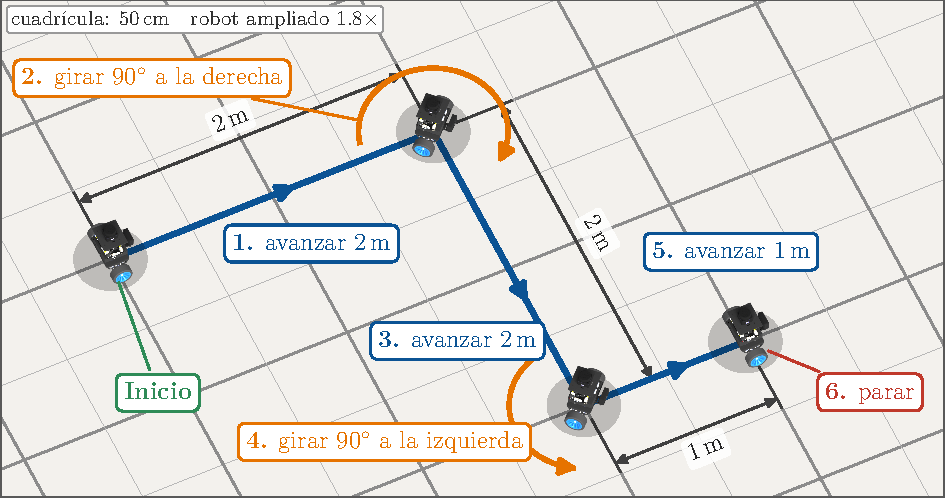
\includegraphics[width=0.6\textwidth]{Images/mision_avanzar_girar2.pdf}
\caption{Misión 1}
\label{mision1}
\end{figure}

El lazo de control está en el archivo \cod{APP/app_control.c}. Para probar una ley de control propia sin modificar ese archivo:
\begin{enumerate}
	\item Copie \cod{APP/app_control.c} con otro nombre, por ejemplo \cod{APP/mi_control.c},
	y haga los cambios en la copia.
	\item Pase el nombre en la llamada:\nopagebreak
	\begin{lstlisting}[nolol]
set_ss_controller(Klqr; mode=0, ref_pos=0.0, file="mi_control.c")
	\end{lstlisting}
	\item Cambie dinámicamente los modos, según sea necesario para cumplir la misión.
\end{enumerate}

\emph{Sugerencia:  es mejor usar los modos de velocidad que usar el modo de balance con referencias de ángulo y posición.}

\section*{Segunda misión: ocho}

Programe los modos de control para que el robot quede describiendo continuamente un 8 como el mostrado en la figura siguiente:
\begin{figure}[H]
	\centering
	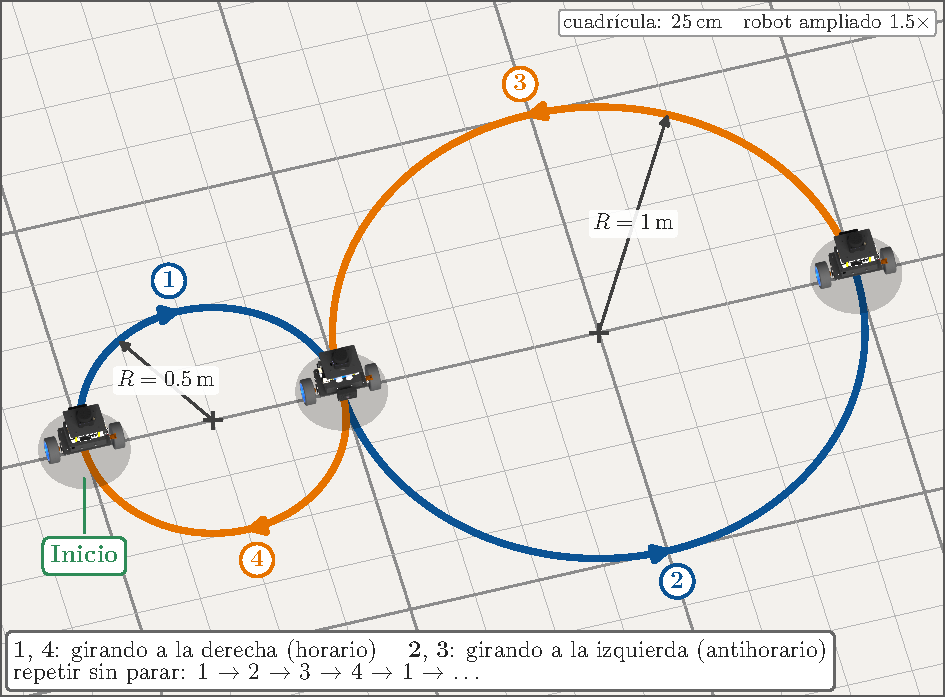
\includegraphics[width=0.6\textwidth]{Images/mision_ocho.pdf}
	\caption{Misión 2}
	\label{mision2}
\end{figure}

\section{Misión 3: evasión de obstáculos}

El que grupo que habiendo cumplido la misión 1 y la 2 se aproxime más al objetivo en la tercera misión, tendrá 5.0 en la nota del segundo parcial. Aqui está la figura: 


\begin{figure}[H]
	\centering
	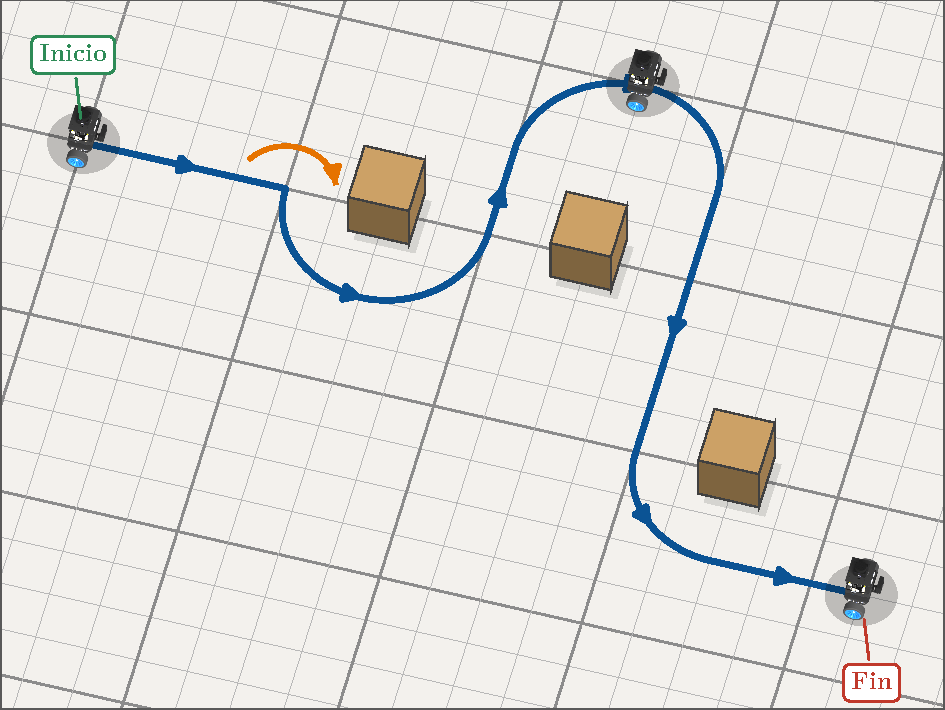
\includegraphics[width=0.6\textwidth]{Images/mision_obstaculos.pdf}
	\caption{Misión 3}
	\label{mision3}
\end{figure}
\end{document}
